%this is chapter about the process of benchmarking cardinality estimation for DBMS

\chapter{BENCHMARKING CARDINALITY ESTIMATION ON POSTGRESQL}\label{chapter:Benchmarking CE}

\section{BASIC THEORIES AND IMPORTANT CONCEPTS}

\subsection{Q-error}

\subsubsection{The Definition of Q-error}

In \cite{q-error}, R and A are respectively a relation and its attributes, and $\left\{x_{1},...,x_{m}\right\}$ = ${{\Pi}_{A}\left(R\right)}$ is the set of distinct values of A. The frequency density is a set of pairs ${\left(x_{i},f_{i}\right)}$ with $f_{i}$ = $\vert{\sigma_{A=x_i}\left(R\right)}\vert$, ${{1}\le{i}\le{m}}$

Define $F$ as a function to approximate this set of paris; $F\left(x_{i}\right)$ =: $F_{i}$ gives the estimate $F_{i}$ of $f_{i}$. And $F$ returns value in a range between 0 and 1.

Typically, norms are used to define the error. $\vec{b}$ = ${{\left(f_{1},...,f_{m}\right)}^{T}}\in{{\mathbb{R}}^{m}}$ organizes the correct values and the estimates into a vector $\vec{B}$ = ${{\left(F_{1},...,F_{m}\right)}^{T}}\in{{\mathbb{R}}^{m}}$. $l_{p}$ error metrics are based on $l_{p}$ norms as in 

\[
\Vert{b-B}\Vert_{p}
\]

where ${{1}\le{p}\le{\infty}}$ and the most common norms are 

\[
{\Vert{z}\Vert}_{2} = \sqrt{{\left(z_{1}\right)}^{2} +...+ {\left(z_{m}\right)}^{2}}
{\Vert{z}\Vert}_{\infty} =  \overset{m}{\underset{i=1}{max}}{\vert{z_{i}}\vert}
\]

for z = ${{\left(z_{1},...,z_{m}\right)}^{T}}\in{{\mathbb{R}}^{m}}$. While the $l_{2}$ error does not give bound on estimates, $l_{\infty}$ does. Define $\Delta$ = ${\Vert{b-B}\Vert}_{\infty}$. Then 

\[
{{f_{i} - \Delta}\le{F_{i}}\le{f_{i} + \Delta}}
\]

However, this error bounds are not really useful in the context of query optimization. For $z\in{\mathbb{R}}$, a multiplicative error:

\begin{subnumcases}{{{\Vert{z}\Vert}_{Q}}=}
    \infty \quad if \quad {z}\le{0}\\
	\frac{1}{z} \quad if \quad {0}<{z}\le{1}  \\
	z \quad if \quad {1}\le{z}    
\end{subnumcases}

For $z>0$, this is the same as saying $\Vert{z}\Vert_{Q}$ = $max\left(z,{\frac{1}{z}}\right)$. Thus, it treats over and underestimates symmetrically. For a vector ${z}\in{{\mathbb{R}^{m}}}$, define:

\[
{\Vert{z}\Vert}_{Q} =  \overset{m}{\underset{i=1}{max}}{\Vert{z_{i}}\Vert}_{Q}
\]

Let $\vec{a}$ and $\vec{b}$ be two vectors in $\mathbb{R}^{m}$ where $b_{i}$. Define $\vec{a}{/}\vec{b}$ = $\frac{\vec{a}}{\vec{b}}$ = $\left({a_1/b_1},...,{a_n/b_n}\right)^{T}$. Then, we can define the q-error of an estimation B of b as

\[\Vert{B/b}\Vert_{Q}\]

As $l_{\infty}$, $l_q$ produces valid, symmetric bounds for individual estimates. Define q = $\Vert{B/b}\Vert_{Q}$. Then,

\[
{\left(\frac{1}{q}\right)f_{i}}\le{F_{i}}\le{q{f_{i}}}
\]

To measure the quality of base table cardinality estimates, q-error is the factor by which an estimate differs from the true cardinality. For example, if the true cardinality of an expression is 1000, the estimates of 10 or 100000 both have a q-error of 100.

\subsection{Logical join operators}

Logical operators \cite{join operators} decribe the relational algebraic operation used to process a statement. In other words, logical operators decribe conceptually what operation needs to be performed. In PostgreSQL. there are logical join operators, such as Inner join, Outer join, Cross join.

\subsubsection{Inner join}

It looks for two rows that satisfy a join predicate. For example, this query used the join predicate "customer.id=salary.customerid" to find all Customer and Sale rows with the same customerid.

\begin{figure}[H]
	\centering
	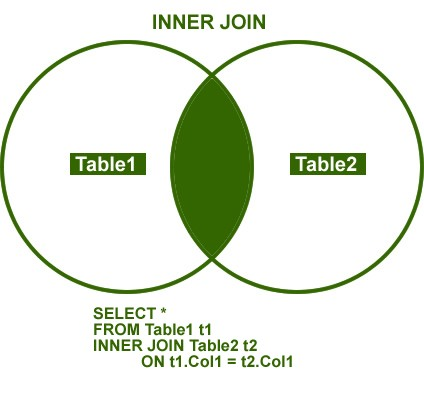
\includegraphics[width=0.5\textwidth]{logical_operators/inner_join.jpg}
	\caption{An example about inner join \cite{figures}.}
\end{figure}

\subsubsection{Outer join}

\begin{itemize}
	\item Left outer join: Its result contains all rows of the "left" table, even if the 				join-condition does not find any matching row in the "right" table. Figure 4.2
		makes more specific about that.
\begin{figure}[H]
	\centering
	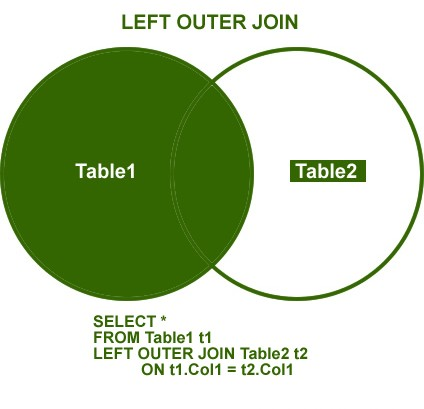
\includegraphics[width=0.5\textwidth]{logical_operators/left_outer_join.jpg}
	\caption{An example about left outer join \cite{figures}.}
\end{figure}

	\item Right outer join: In contrast with left outer join, the result of right outer join 		contains all rows of the "right" table, even if the join-condition does not find any 		matching row in the "left" table. Figure 4.3 shows that:

\begin{figure}[H]
	\centering
	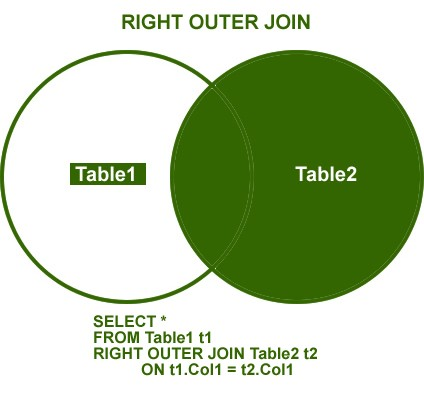
\includegraphics[width=0.5\textwidth]{logical_operators/right_outer_join.jpg}
	\caption{An example about right outer join \cite{figures}.}
\end{figure}

	\item Full outer join: A full outer join combine left outer join and right outer 					join. So, the result of full outer join contains all rows of both tables. With the 				lack of a matching row, the result set will have NULL values for every column of the 		table. 

\begin{figure}[H]
	\centering
	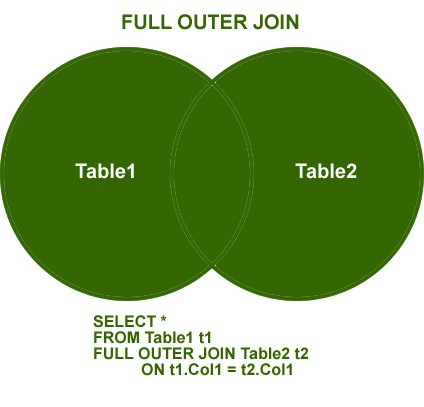
\includegraphics[width=0.5\textwidth]{logical_operators/full_outer_join.jpg}
	\caption{An example about full outer join \cite{figures}.}
\end{figure}

\end{itemize}

\subsubsection{Cross join}

If where clause is not used, the result set of the cross join is the number of rows in the first table multiplied by the number of rows in the second table; whereas it functions like an INNER JOIN.

\subsection{Physical join operators}

Physical join operators are used by DBMSs internally to implement these logical join operators, DBMSs use three different physical operators. Three physical join operators are respectively Nested Loops Join, Hash Join, Merged Join

\subsubsection{Nested Loops Join}

In Nested Loops join \cite{physical operators}, for each iteration of the outer loop all the iterations of the inner loop are executed. To be more specific, for each row of the outer table, all rows from the inner table are examined with this row. If matched, the row from the inner table is included in the result-set; whereas it is ignored. The next row from the outer table is picked up and the same process is repeated.

In terms of complexity, If N is the number of rows from the outer output and the number of rows that table is M. The complexity of this join operator is O(N*M). Therefore, The PostgreSQL's optimizer might choose a Nested Loops join when  one of the joining tables is small (considered as the outer table) and another one is large (consider as the inner table).

\subsubsection{Merge Join}

In Merge join \cite{physical operators}, the inputs are required to be sorted on join keys/merge columns. As a consequence of being sorted, this join operator reads a row from one input and then compares it with the row of another input. If the rows match, that matched row is included in result set and then it reads the next row from the input table; whereas the lesser of the two rows is ignored and the process continues this way until all rows have been processed.

In terms of complexity, it is assumed that N, M are the row numbers of tables, the complexity of this join operator is O(N+M). If the inputs are not both sorted on the join key, the PostgreSQL optimizer will not choose the Merge join type due to the the cost of pre-sorting process.

\subsubsection{Hash join}

There are two phases in a hash join \cite{physical operators}. They are the build phase and the probe phase; so it has two inputs called build input and proble input. It is considered that the smaller table is build input and the other one is probe input.

In the build phase, join keys of all the rows from the build table are scanned and then hashes are generated and stored in hash table. In the probe phase, join keys of each row of the probe table are scanned and hashes are generated again, then compared against the corresponding hash table for a match.

Hash table requires memory resource to store and a hash function requires significant amount of CPU cycles to generate hashes. To achieve high performance, the PostgreSQL optimizer may parallelize a Hash join to scale better than any other join.

In term of complexity, it is assumed that $h_c$ is the complexity of the hash table creation, and $h_m$ is the complexity of the hash match function. Therefore, the complexity of the Hash join will be O(N*$h_c$ + M*$h_m$ + J) where N is the smaller data set, M is the larger data set and J is a “joker” complexity addition for the dynamic calculation and creation of the hash function.

\section{BENCHMARKING}

I use JOB benchmark queries to examine the q-error of Postgresql estimator's cardinality estimation. The volume of JOB data set is about 20GB. Figure 4.5 shows the q-error of plan node by its join level. Figure 4.6 shows the q-error of plan node per query. Figure 4.7 and figure 4.8 show respectively the q-error of plan node by join tree depth, the comparison between actual execution time and estimated execution time of queries.

\begin{figure}[H]
	\centering
	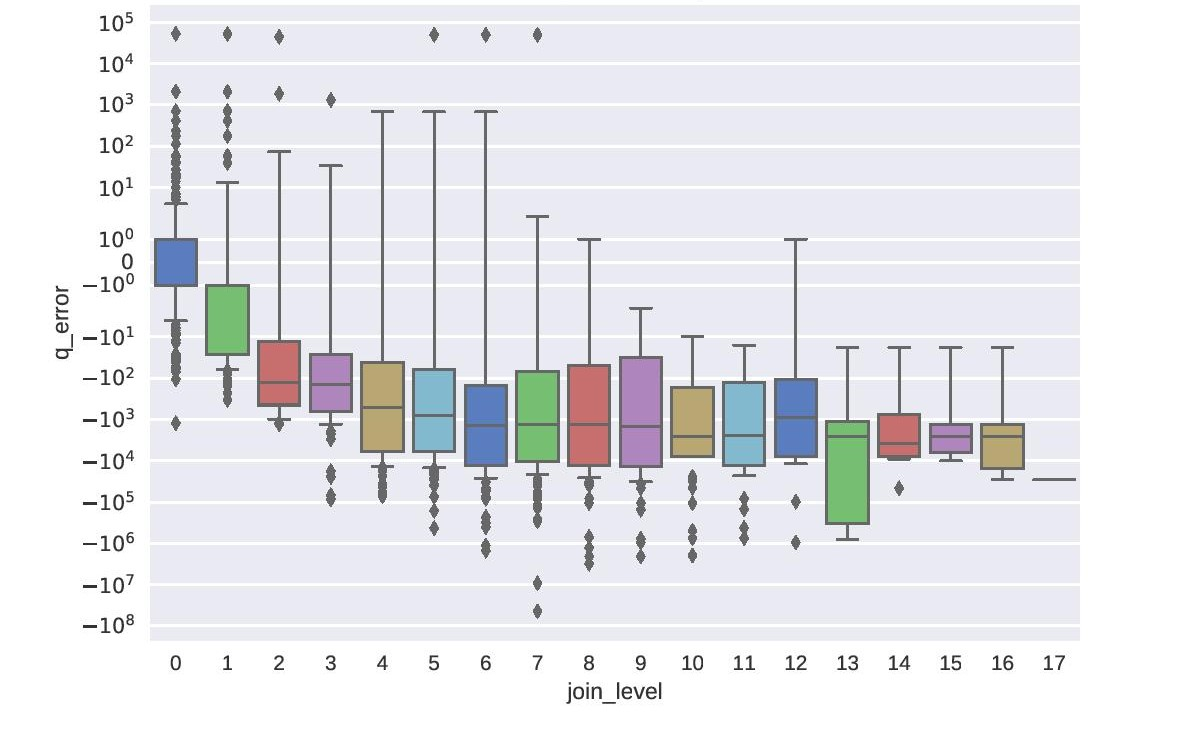
\includegraphics[width=1.0\textwidth]{results/plan_node_q-error.jpg}
	\caption{Q-error of plan node and its join level.}
\end{figure}

\begin{figure}[H]
	\centering
	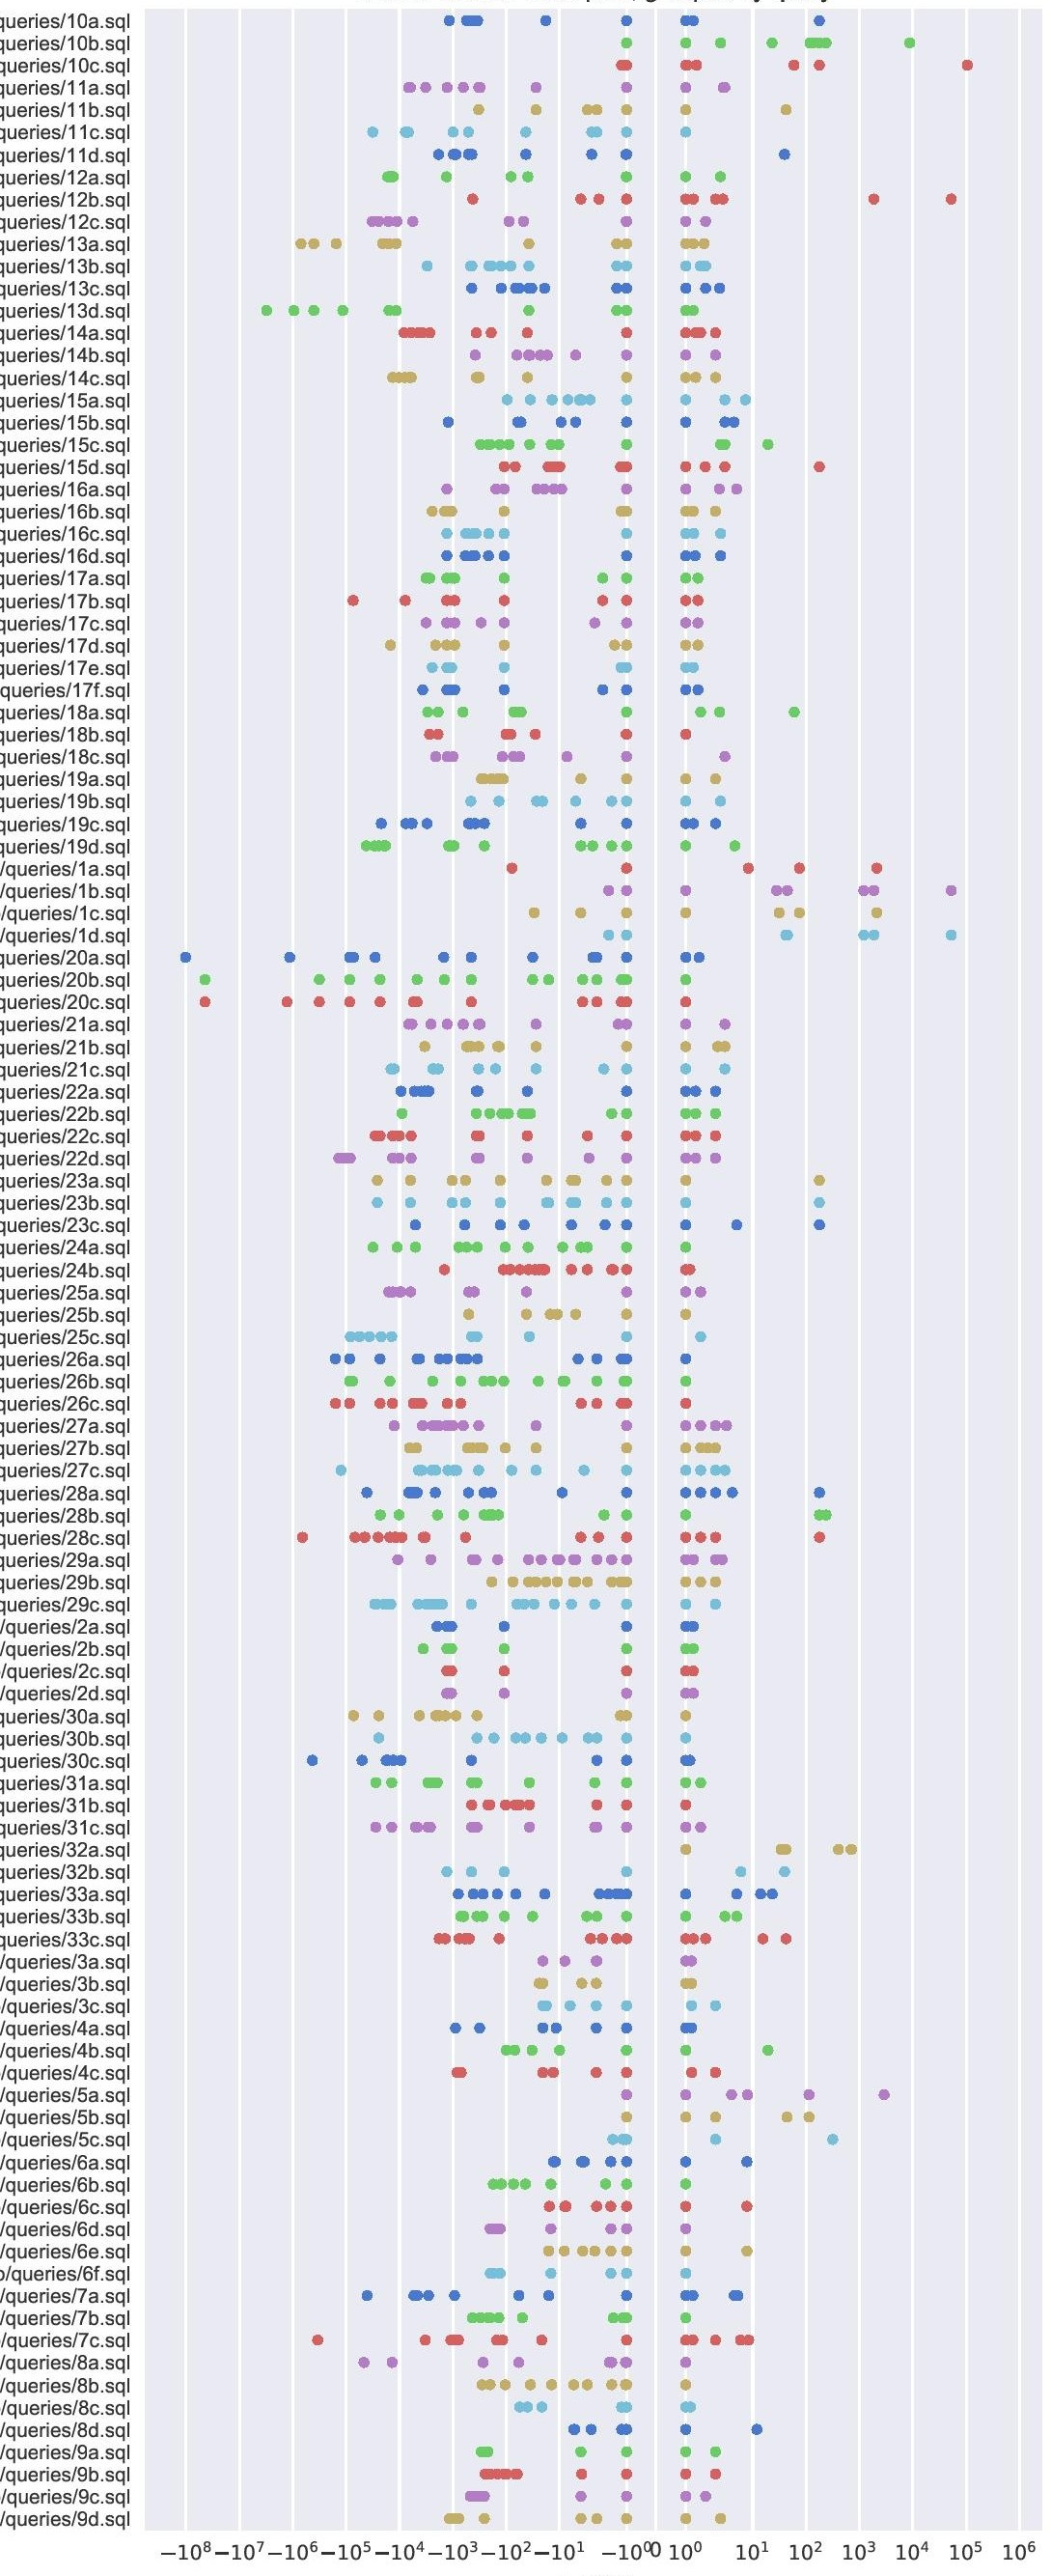
\includegraphics[width=0.65\textwidth]{results/q-error_per_query.jpg}
	\caption{Q-error of plan node per query.}
\end{figure}

\begin{figure}[H]
	\centering
	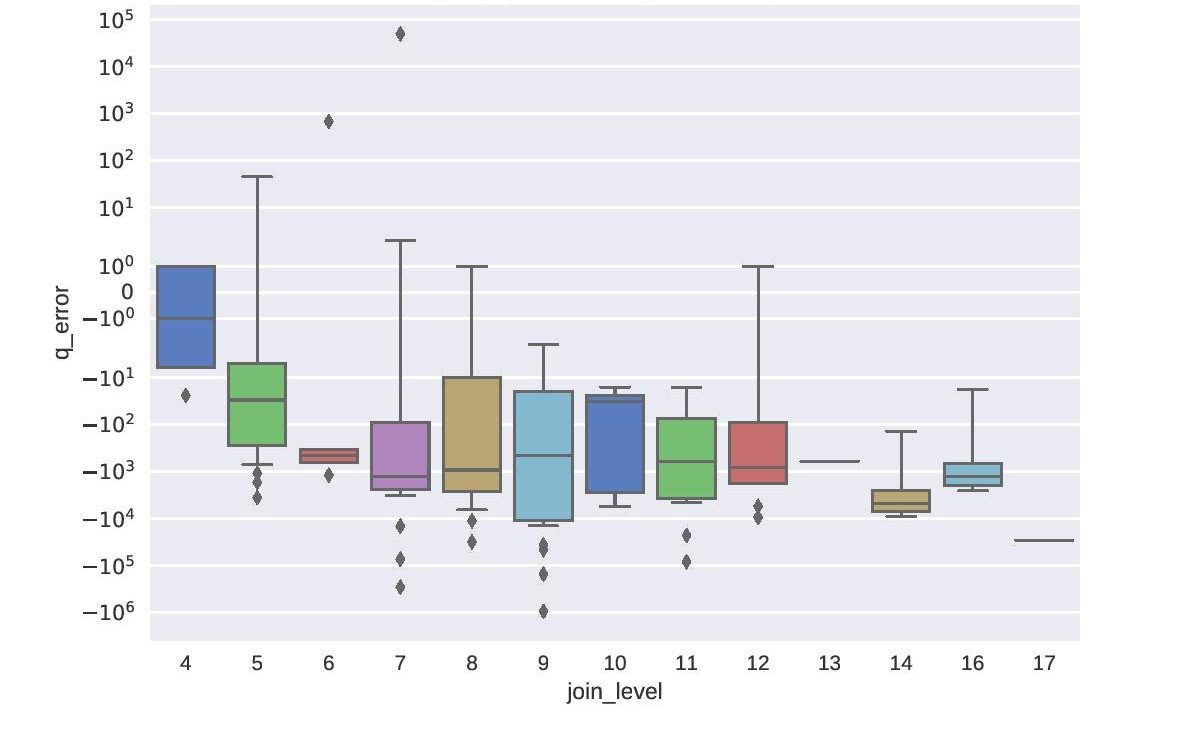
\includegraphics[width=1.0\textwidth]{results/plan_node_q-error_join_tree_depth.jpg}
	\caption{Q-error of plan node and join tree depth.}
\end{figure}

\begin{figure}[H]
	\centering
	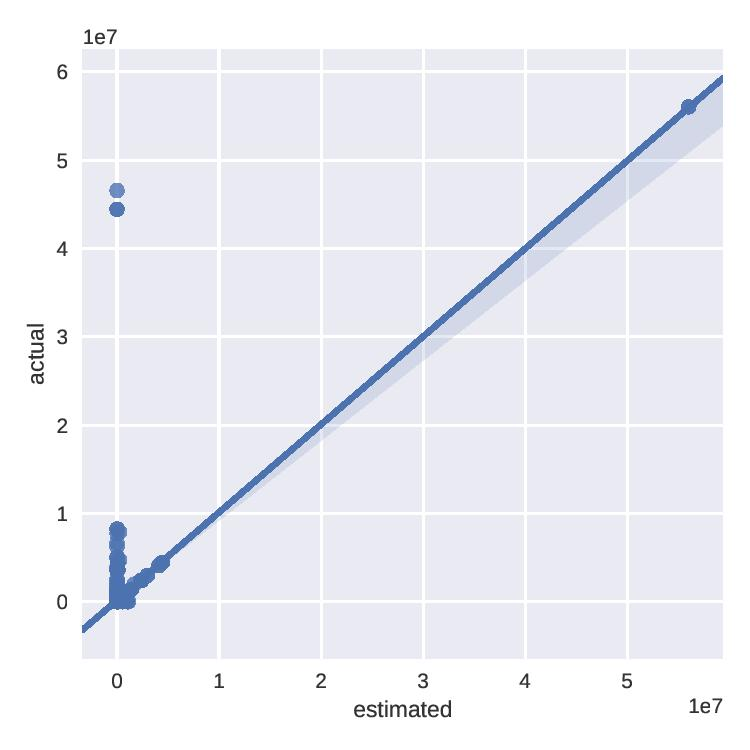
\includegraphics[width=1.0\textwidth]{results/actual_time_and_estimated_time.jpg}
	\caption{actual execution time and estimated execution time.}
\end{figure}

\section{ANALYZING THE EFFECT OF BAD CARDINALITY ESTIMATION} 

As i mentioned in chapter 2, PostgreSQL optimizer is a purely cost-based optimizer. Therefore, when the cost is misestimated, it  leads to that PostgreSQL doesn't choose the plan with smallest cost. The example below shows the effect of estimation to which plan the PostgreSQL's optimizer chooses :
\begin{itemize}
	\item A, B are two relations; $card\left(A\right)_{est}$, $card\left(B\right)_{est}$ are 		respectively cardinality estimation of A,B; $card\left(A\right)_{real}$, $card					\left(A\right)_{real}$ are respectively true cardinality of A, B.
	
		\[
		card\left(A\right)_{est} = 1000, card\left(B\right)_{est} = 1
		\]
		\[
		card\left(A\right)_{real} = 1000, card\left(B\right)_{real} =  1000
		\]

\begin{table}[ht]
\begin{center}
\begin{tabular}{|c|c|}
	\hline
	A nested loop join B  & A merge join B\\
	\hline
	complexity = O(n*m) & complexity = O(n+m)\\
	\hline 
	estimated cost = 1000 * 1 = 1000 & estimated cost = 1000 + 1 = 1001\\ 
	\hline 
	actual cost = 1000 * 1000 = 1000000 & actual cost = 1000 + 1000 = 2000\\ 
	\hline 
\end{tabular}
\end{center}
\label{tab:dum1}
\caption{Operators sensitivity to estimation errors.}
\end{table}
\end{itemize}

The underestimation of PostgreSQL's estimator in this example is 1000. Look at the table, we find that the estimated cost of nestedloop join is smaller than the estimated cost of merge join, so the planner's choice is nestedloop join instead of merge join whose actual cost is smaller about 1000 times than nestedloop join. 

Figure 4.5, figure 4.6, figure 4.7, we find that most of the cardinality estimation of PostgreSQL estimator on JOB queries is underestimation. As a consequence of this underestimation, PostgreSQL's optimizer decides to introduce a nestedloop join because of a very low cardinality estimate, whereas in fact the true cardinality is larger, which lead PostgreSQL's optimizer to choose worse plan. Therefore, query performance is decreased remarkably. To demonstrate this, i make the comparision between query performance between PostgreSQL with and without nestedloop join on JOB benchmarks. 

\newpage
\begin{figure}[H]
	\centering
	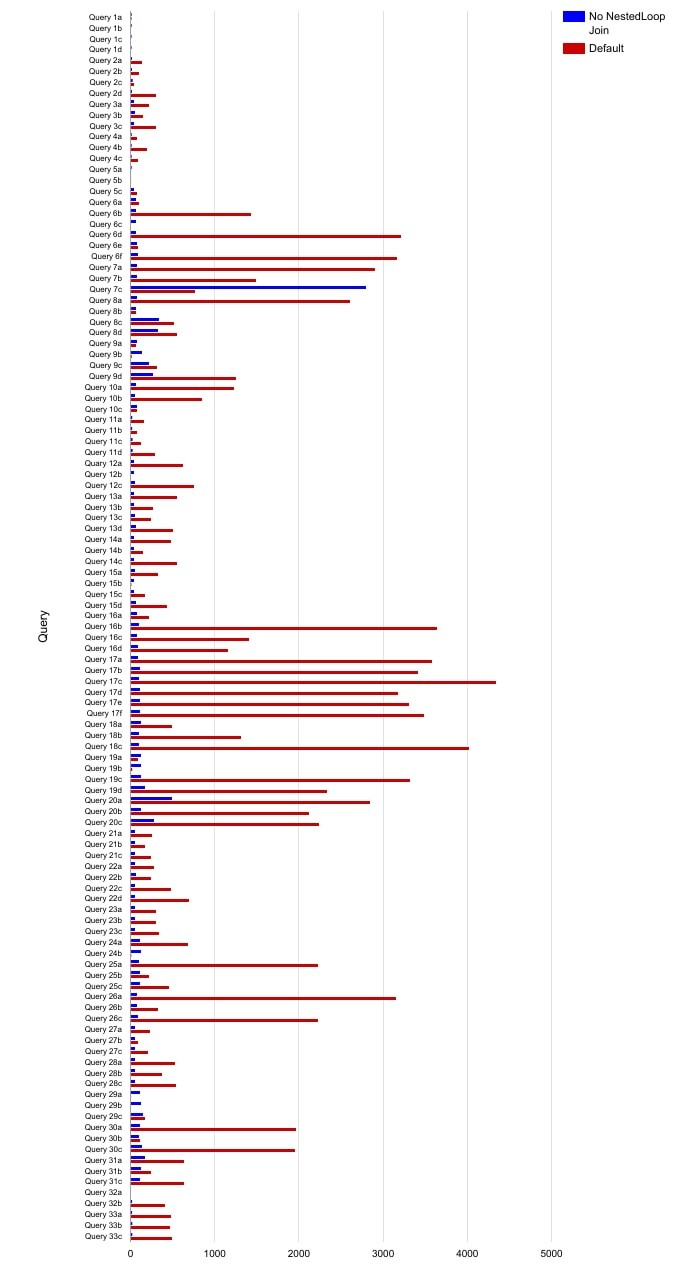
\includegraphics[width=0.85\textwidth]{results/executiontime.jpg}
	\caption{Query execution time (s) between  PostgreSQL with and without nestedloop join.}
\end{figure}

As Figure 4.9 shows, when rerunning all queries of JOB benchmarks without the risky nested-loop joins, we observed that the queries's execution time are improved significantly. For example, The execution time of query 6d is smaller 44 times after rerunning all queries of JOB benchmarks without the risky nested-loop joins, which declines from about 3213 seconds to nearly 73 seconds.

\section{THE PUBLISHED SOLUTIONS}

There have been many solution published to improve the query performance. There are some lines of these solutions.

\begin{itemize}
	\item Use machine learning methods for cardinality estimation. For example:
	\begin{itemize}
		\item In \cite{adaptive cardinality estimation} the main point of their approach is 				using query execution statistics of previously queries to improve cardinality 					estimations. It is called adaptive cardinality estimation.
		\item In \cite{neural network approach} neural networks are used to estimate the 					selectivity for user defined functions and data types. Nevertheless, this paper 				address the problem of estimation the selectivity for a single clause.
		\item In \cite{probabilistic models} it is proposed to estimate node selectivity 					using inference in automatically constructed Bayesian networks. 
	\end{itemize}
	\item Use sampling-based approach \cite{sampling-based,cost models are unusable}. They 				do not improve query optimizer's cost estimator directly, but propose sampling-based 		ways to rectify standard query optimizer's errors if they are. Sampling-based 					approches are good on low-relational queries, but on queries with lots of joins they 		may have too large variance.
	\item Use multidimensional statistics for correct cardinality estimation \cite{A 					multidimensional workload-aware histogram,multidimensional range queries}. Instead 				of using single histogram as in DBMSs, multidimensional histograms are used. It is 				the most popular way to improve standard cardinality estimation method in DBMS 					community.
\end{itemize}

